\documentclass[crop,tikz]{standalone}
\usetikzlibrary{backgrounds}
\colorlet{blue}{cyan}
\tikzset{
  inverted/.style = {
    color=white,
    background rectangle/.style={fill},
    show background rectangle
  }
}

\usepackage{pgfplots}
\colorlet{green}{green}

\tikzset{>=latex}

\pgfplotsset{
  every non boxed x axis/.append style={
    axis line style={-latex}
  },
  every non boxed y axis/.append style={
    axis line style={-latex}
  },
  inverted/.style = {
    every axis legend/.append style={
      draw=white,
      fill=black,
      text=white
    }
  }
}

\begin{document}
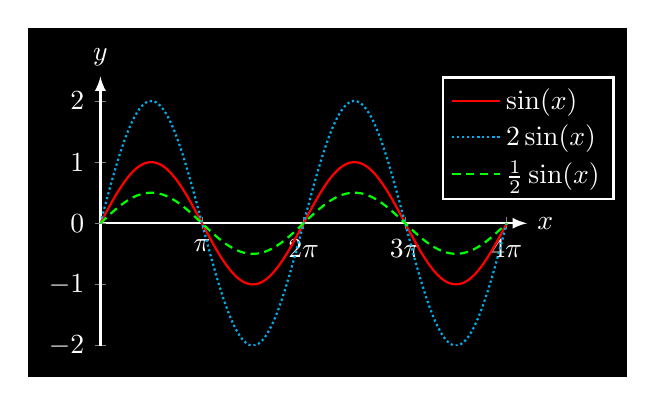
\begin{tikzpicture}[inverted,inverted]
\begin{axis}[inverted,
  thick,
  width=7cm,
  height=5cm,
  domain={0}:{4*pi},
  samples=100,
  smooth,
  axis y line=middle,
  axis x line=middle,
  xlabel={$x$},
  ylabel={$y$},
  xlabel style={right},
  ylabel style={above},
  xmin=0, xmax={4.2*pi},
  ymin=-2, ymax=2.4,
  xtick={0, pi, 2*pi, 3*pi, 4*pi},
  xticklabels={$0$, $\pi$, $2\pi$, $3\pi$, $4\pi$},
  ytick distance=1,
  extra y ticks={0},
  legend cell align={left},
  legend style={at={(0.8,1)},anchor=north west},
  ]
  \addplot[red] { sin(deg(x)) };
  \addlegendentry{$\sin(x)$};
  \addplot[blue,densely dotted] { 2*sin(deg(x)) };
  \addlegendentry{$2\sin(x)$};
  \addplot[green,densely dashed] { 0.5*sin(deg(x)) };
  \addlegendentry{$\frac{1}{2}\sin(x)$};
\end{axis}
\end{tikzpicture}
\end{document}
